\documentclass[12pt,a4paper]{article}
\usepackage[latin1]{inputenc}
\usepackage{amsmath}
\usepackage{amsfonts}
\usepackage{amssymb}
\usepackage{makeidx}
\usepackage{graphicx}
\usepackage[left=2cm,right=2cm,top=2cm,bottom=2cm]{geometry}

\begin{document}
\title{\textbf{Sistemas electronicos de interfaz \\ Tarea 3 \\ EV 2.2. Explicar los arreglos y parametros de los amplificadores clase A}}

\author{Josue Natanael Orozco Nevares 18311797 \\ Ing. Mecatronica 4 B}
\date{1 de Octubre del 2019}
\maketitle

\begin{figure}[h!]
\centering

\includegraphics[width=10cm]{UPCDLZMDG5783-logo.png} 
\end{figure}

\newpage

\section{Introduccion}
En esta investigacion, indagaremos acerca de los amplificadores de clase A, desde su funcionamiento hasta las ventajas y desventajas que estos mismos pueden ofrecer.

\section{Amplificadores de clase A}
Este tipo de amplificadores tienen diferentes etapas de potencia, consumen corrientes altas y continuas de la fuente de alimentacion a la que esten conectados, independientemente de si existe audio o no.

\begin{figure}[h!]
\centering
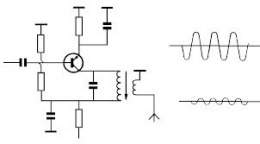
\includegraphics[scale=1]{260px-AmplificadorclaseA.jpg} 
\end{figure}

\subsection{Caracteristicas}
Las caracteristicas de este tipo de amplificadores es que generan una fuerte y constante emision de calor. Los transistores de salida siempre estan a una temperatura fija y sin alteraciones. Por lo general este tipo de amplificacion es muy frecuente en circuitos que tienen que ver con el audio y en equipos domesticos de gama alta, ya que proporcionan calidad de sonido potente y de muy buena calidad.
Por lo general este tipo de amplificadores consisten en un transistor de salida conectado al dispositivo de la fuente de alimentacion y un transistor de corriente constante conectado de la salida al negativo de la fuente de alimentacion.
La senal de dicho transistor de salida modula tanto el voltaje como la corriente de salida. En dado caso de no tener senal de entrada, la corriente de polarizacion fluye directamente del positivo de la fuente al negativo gastandose asi demasiada corriente. Algunos de los amplificadores de clase A mas sofisticados tienen dos transistores de salida en configuracion push-pull.

\subsection{Ventajas}
La clase A de amplificadores se refiere a una etapa de salida con una corriente de polarizacion mayor que la maxima corriente de salida que dan, de tal forma los transistores de salida siempre estan consumiendo corriente, la gran ventaja de esta clase es que es casi lineal y en consecuencia la distorcion es menor.

\subsection{Desventajas}
La gran desventaja de la clase A es que es poco eficiente, se requiere un amplificador de clase A muy grande para dar 50 W, y ese amplificador usa mucha corriente y se pone a muy alta temperatura.

\section{Conclusion}
La utilidad que se le puede dar a estos circuitos o amplificadores clase A es algo basta para la vida cotidiana debido que estos estan implementados en las bocinas que utilizamos comunmente para escuchar ya sea musica entre otras cosas, es increible el saber este tipo de cosas y de lo ignorantes que somos de vez en cuando. Se necesita seguir investigando.

\begin{thebibliography}{10}
\bibitem{Malvino} Malvino, A. P. Bates, D. J. \emph{Principios de electronica} Vol. 2, p. 34. McGraw Hill

\end{thebibliography}



\end{document}